\chapter{Harmonogram realizacji projektu}

W celu kontroli realizacji projektu wykonałem diagram Ganta, biorąc pod uwagę najważniejsze kamienie milowe, podczas tworzenia projeku użyty został system kontroli wersjii Git:
\begin{itemize}
  \item Utworzenie bazy danych 
  \item Planowanie projektu 
  \item Tworzenie i debugging projektu 
  \item Weryfikacja działania aplikacji
  \item Pisanie dokumentacji
\end{itemize}

\begin{figure}[h!]
    \centering
    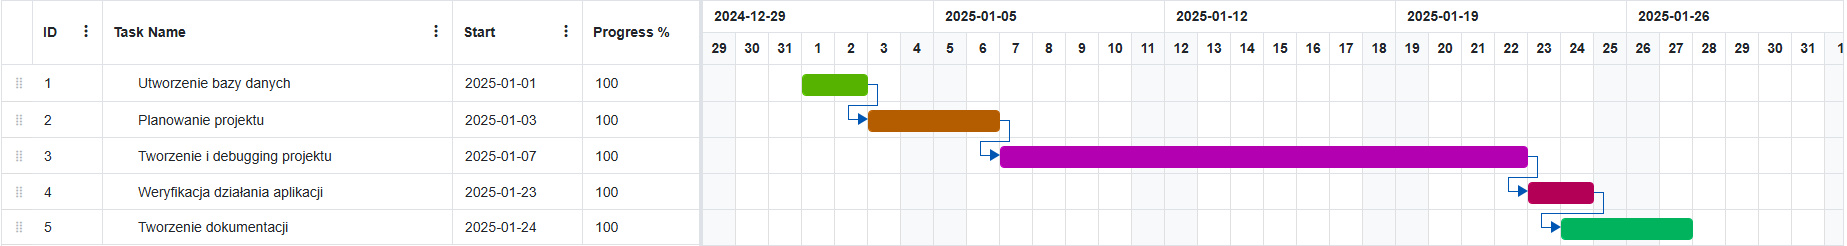
\includegraphics[width=1.2\textwidth]{Diagram Ganta projekt.png}
    \caption{Diagram przedstawiający hierarchię klas w projekcie.}
\end{figure}

Po zakończeniu procesu tworzenia, debuggingu i weryfikacji projektu umieszczony został on na platformie GitHub, pod linkiem : https://github.com/Kacgon/Paczkomat
